\chapter{Screen Blockchain Explorer}
\label{app:a}
Alcuni screen dell'applicazione Blockchain Explorer.

\begin{figure}[H]
	\centering
	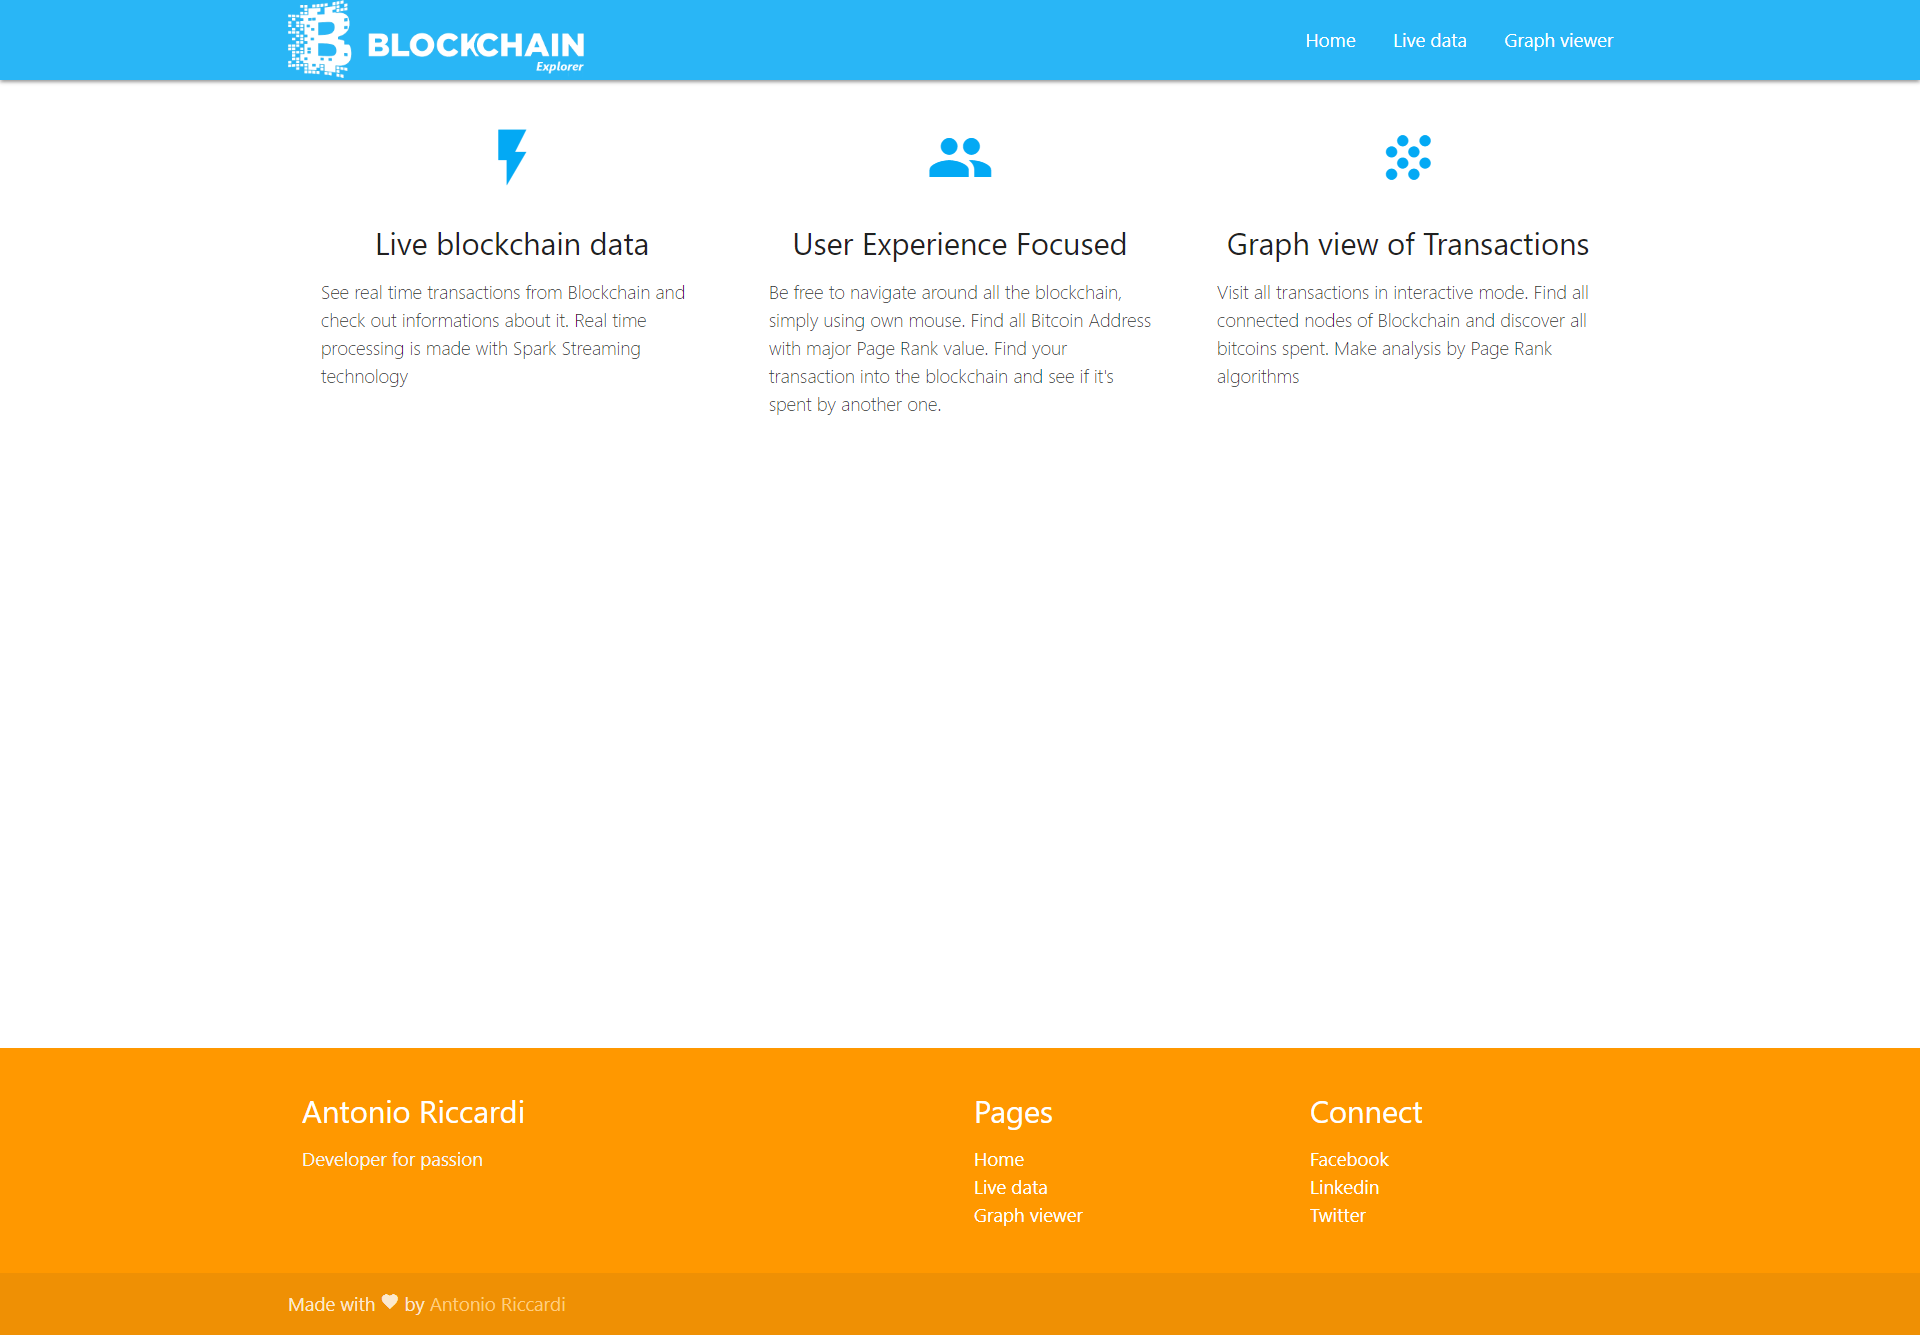
\includegraphics[width=\textwidth, height=0.60\textheight]{images/homePage.png}
	\caption{Home page Blockchain Explorer.}
	\label{fig:homeBE}
\end{figure}

%TODO manca foto elenco transazioni
\begin{figure}[H]
	\centering
	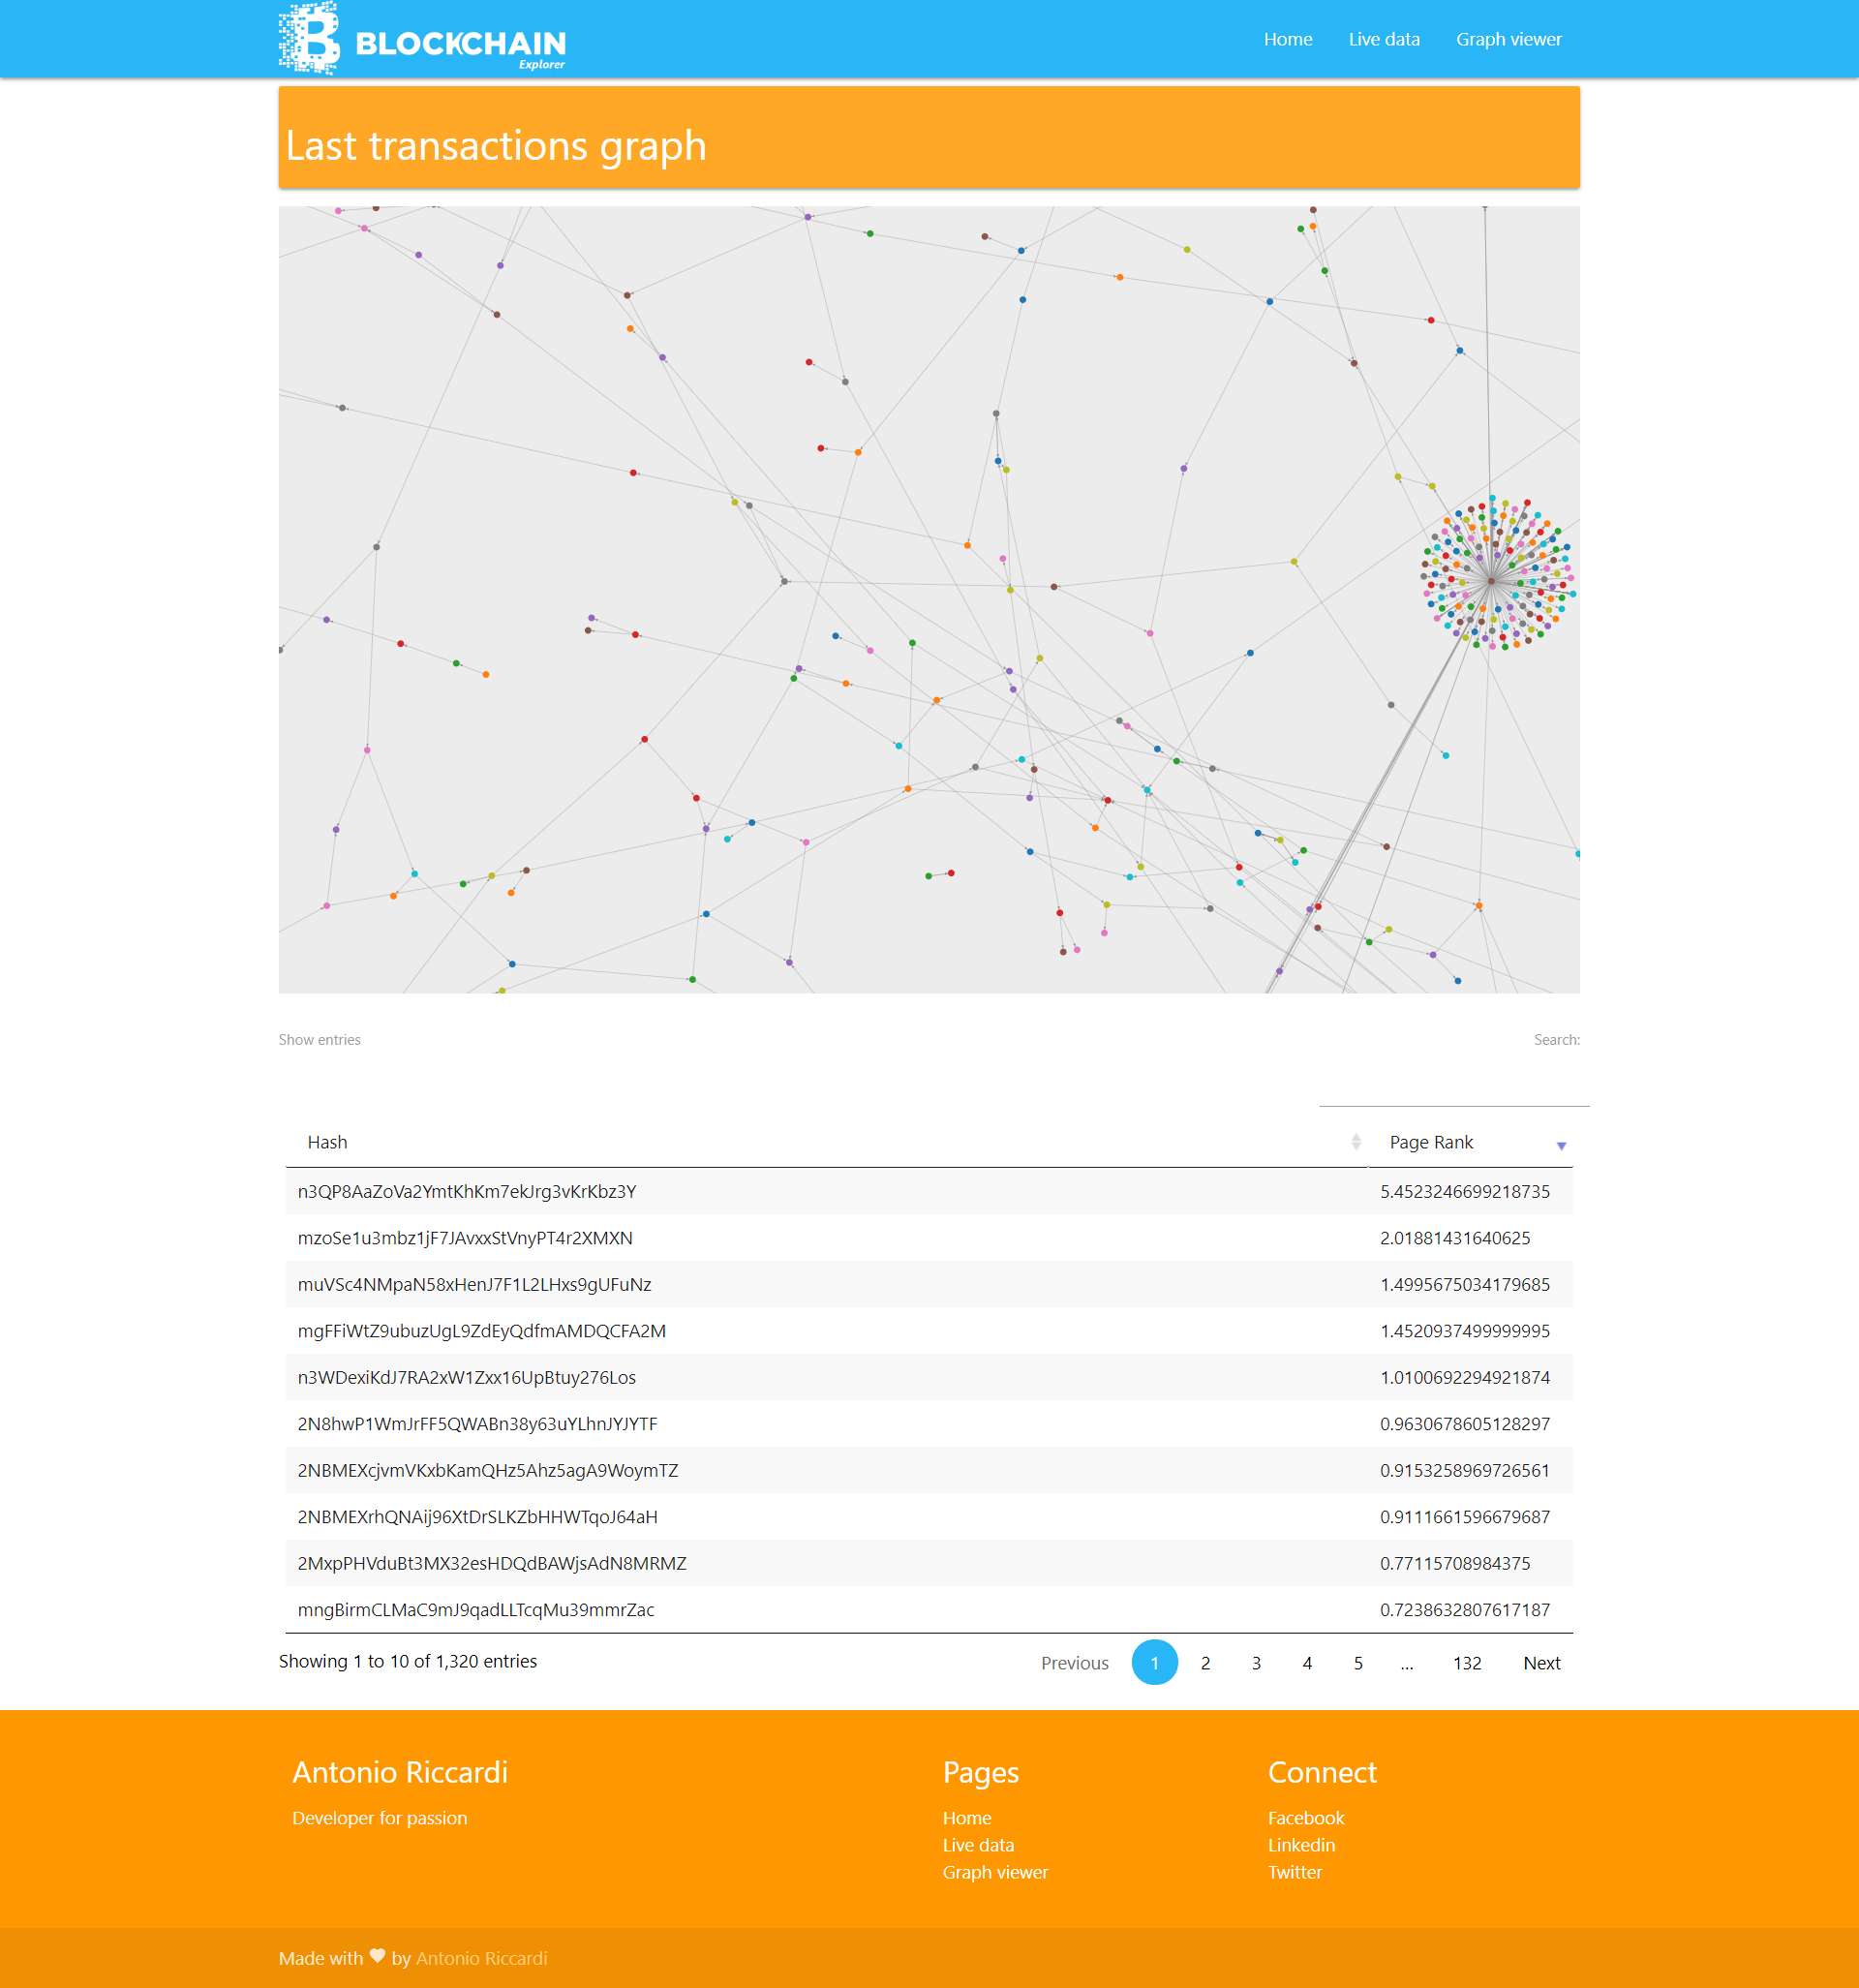
\includegraphics[width=\textwidth, height=0.80\textheight]{images/graphView.png}
	\caption{Elenco ultime transazioni.}
	\label{fig:transactionsBE}
\end{figure}


\begin{figure}[H]
	\centering
	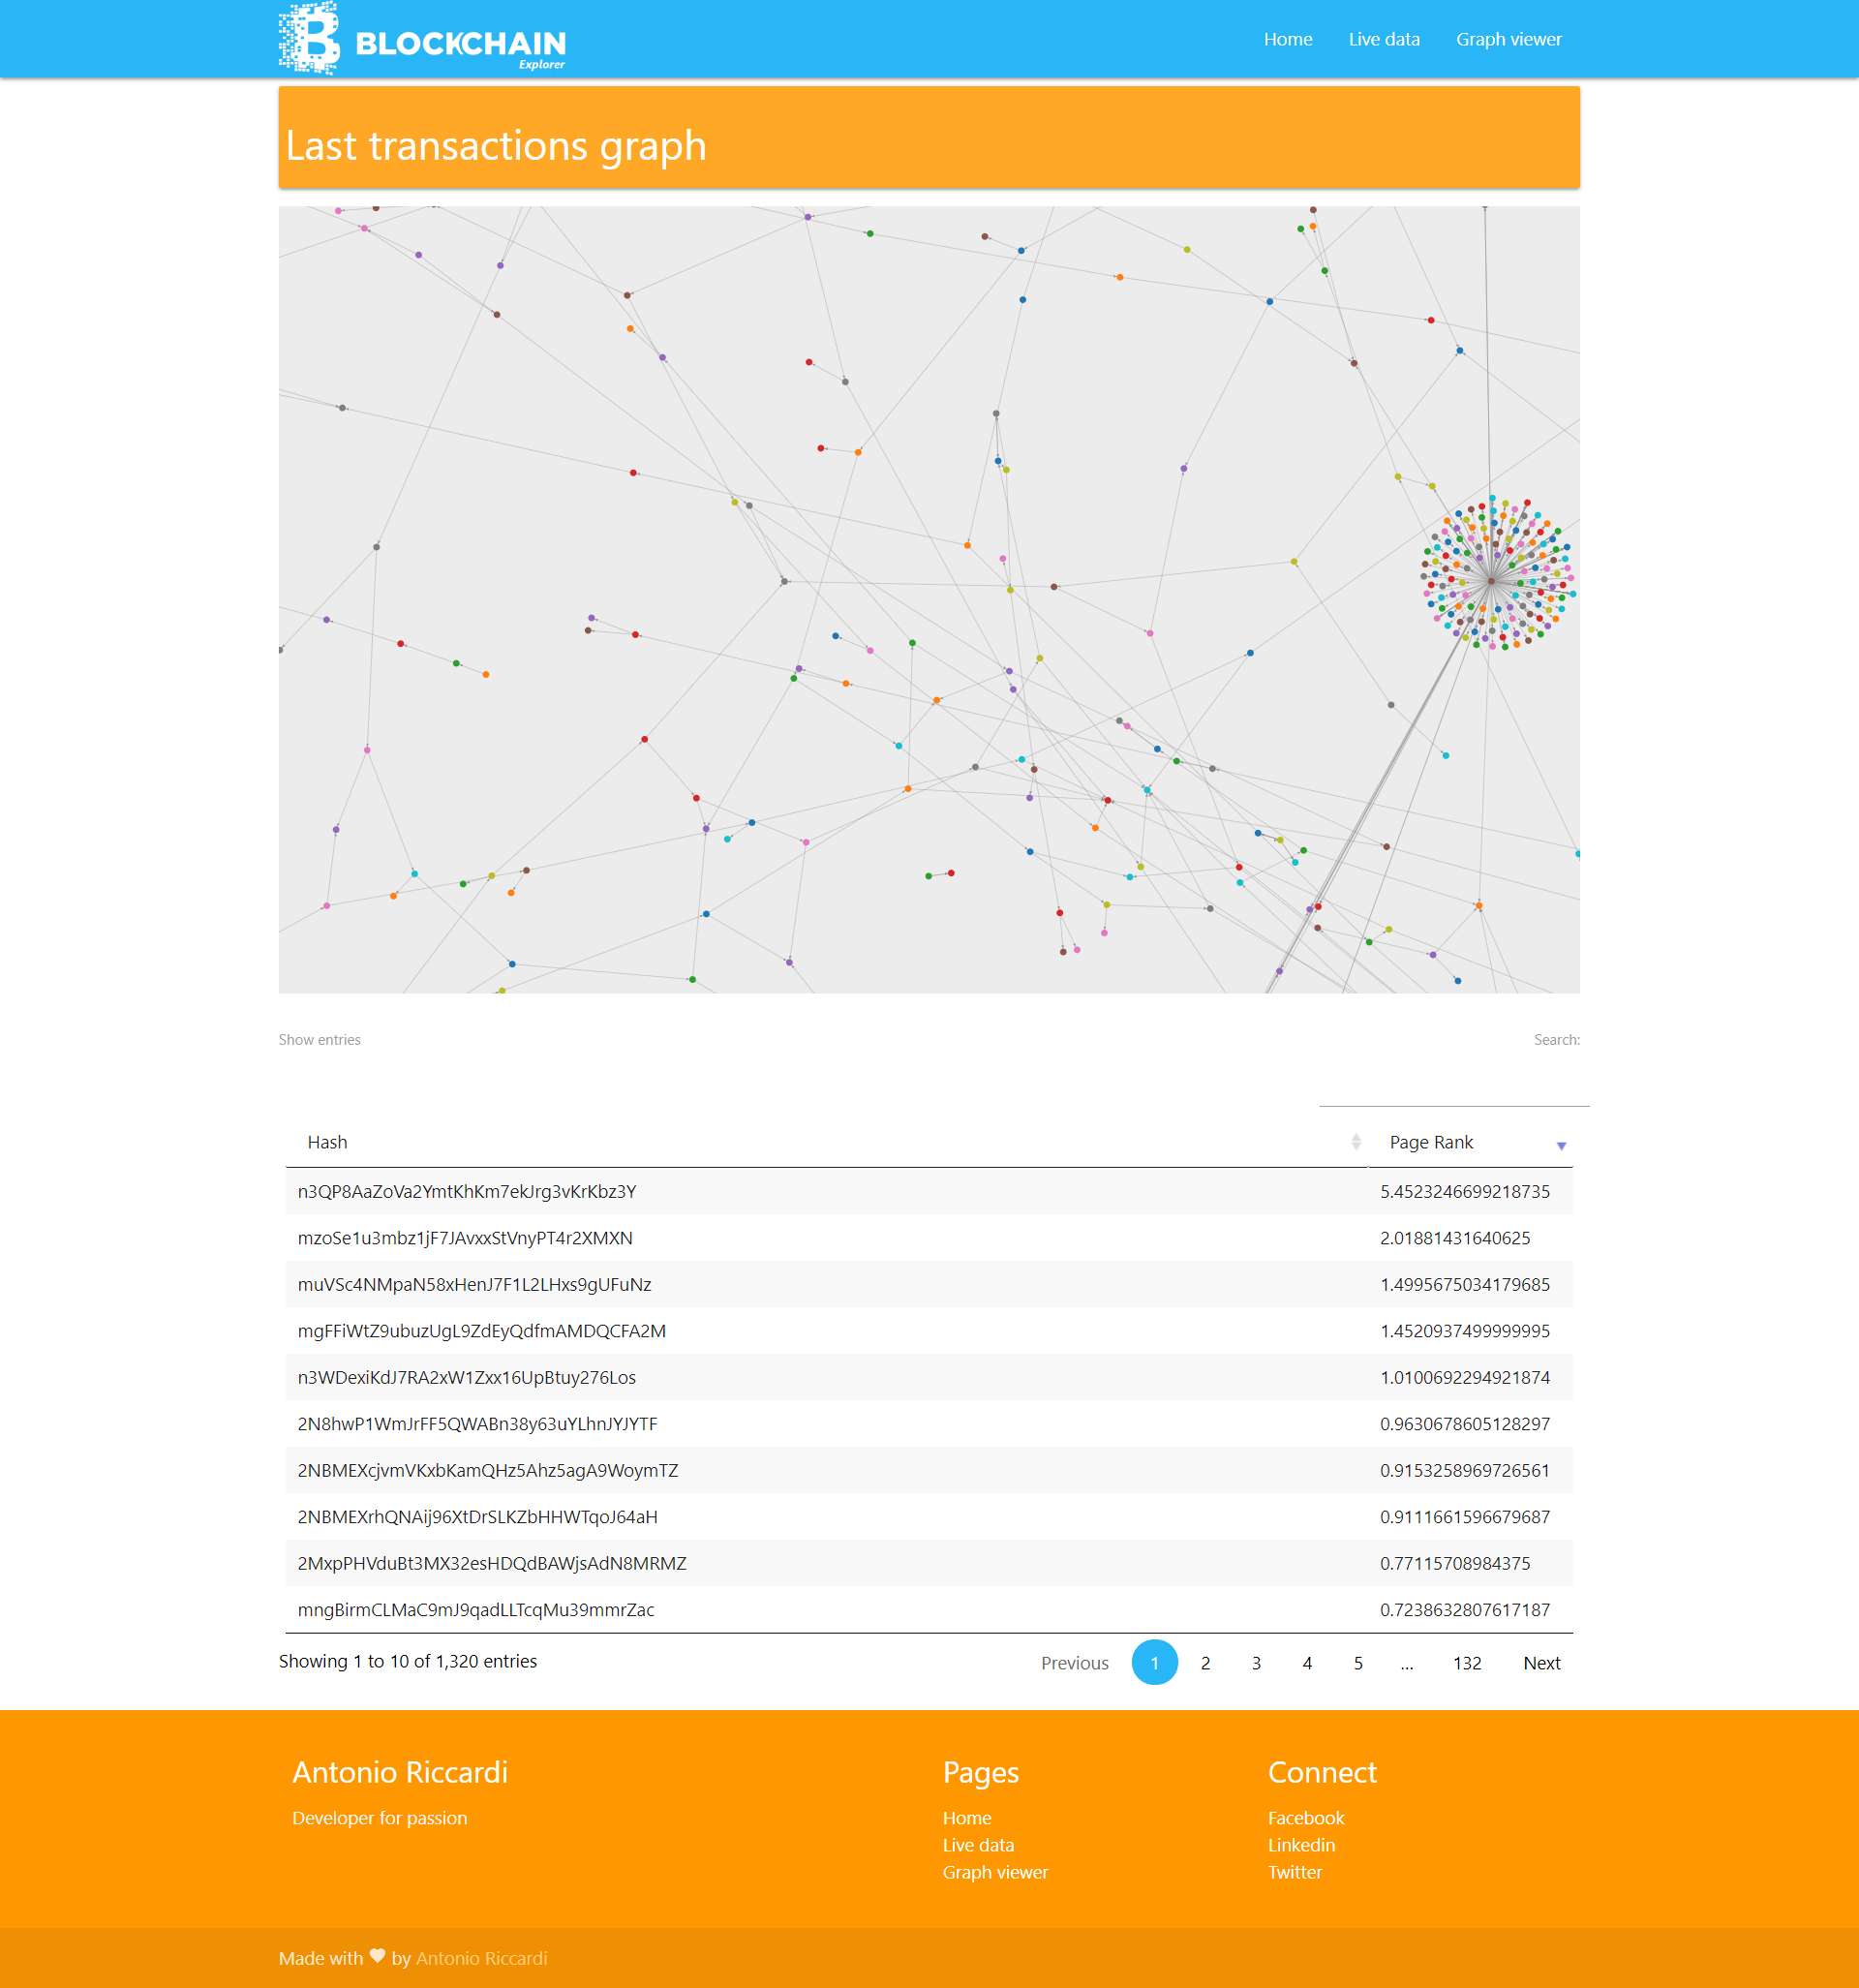
\includegraphics[width=\textwidth, height=0.80\textheight]{images/graphView.png}
	\caption{Visualizzazione intero grafo.}
	\label{fig:graphBE}
\end{figure}

\begin{figure}[H]
	\centering
	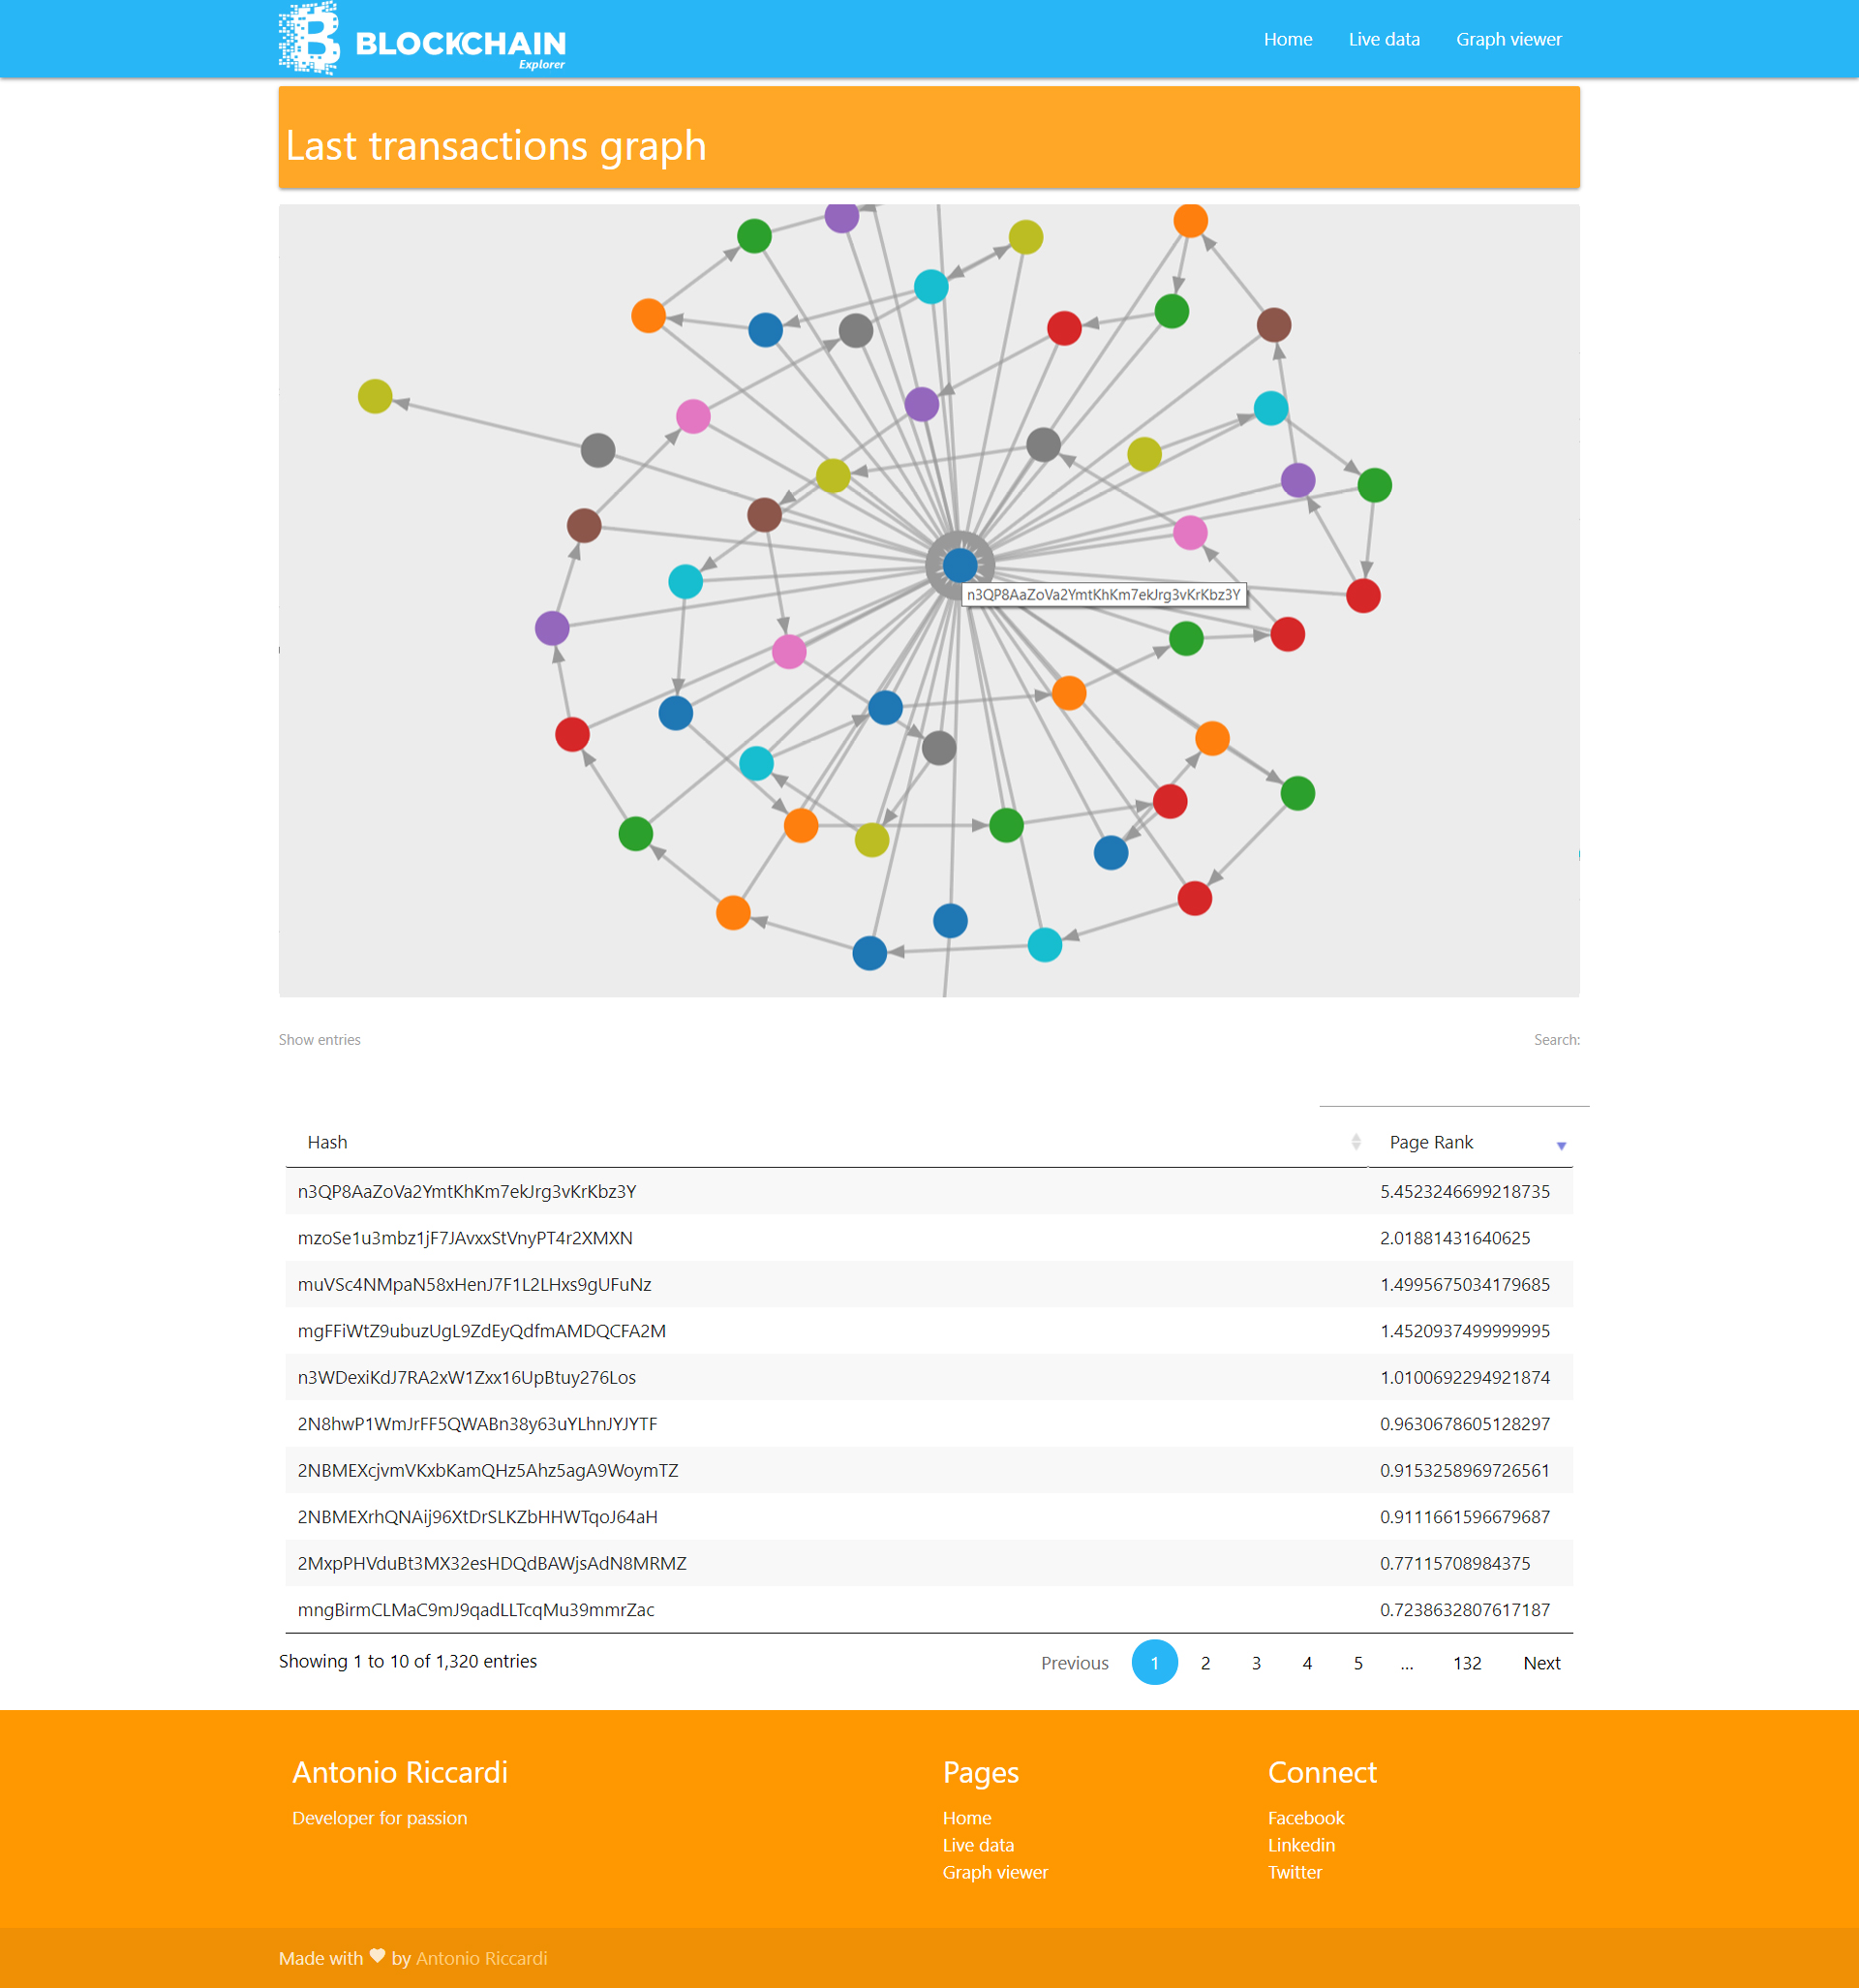
\includegraphics[width=\textwidth, height=0.80\textheight]{images/lastGraph-1.jpg}
	\caption{Dettaglio nodo centrale con Page Rank più alto.}
	\label{fig:graph1BE}
\end{figure}

\begin{figure}[H]
	\centering
	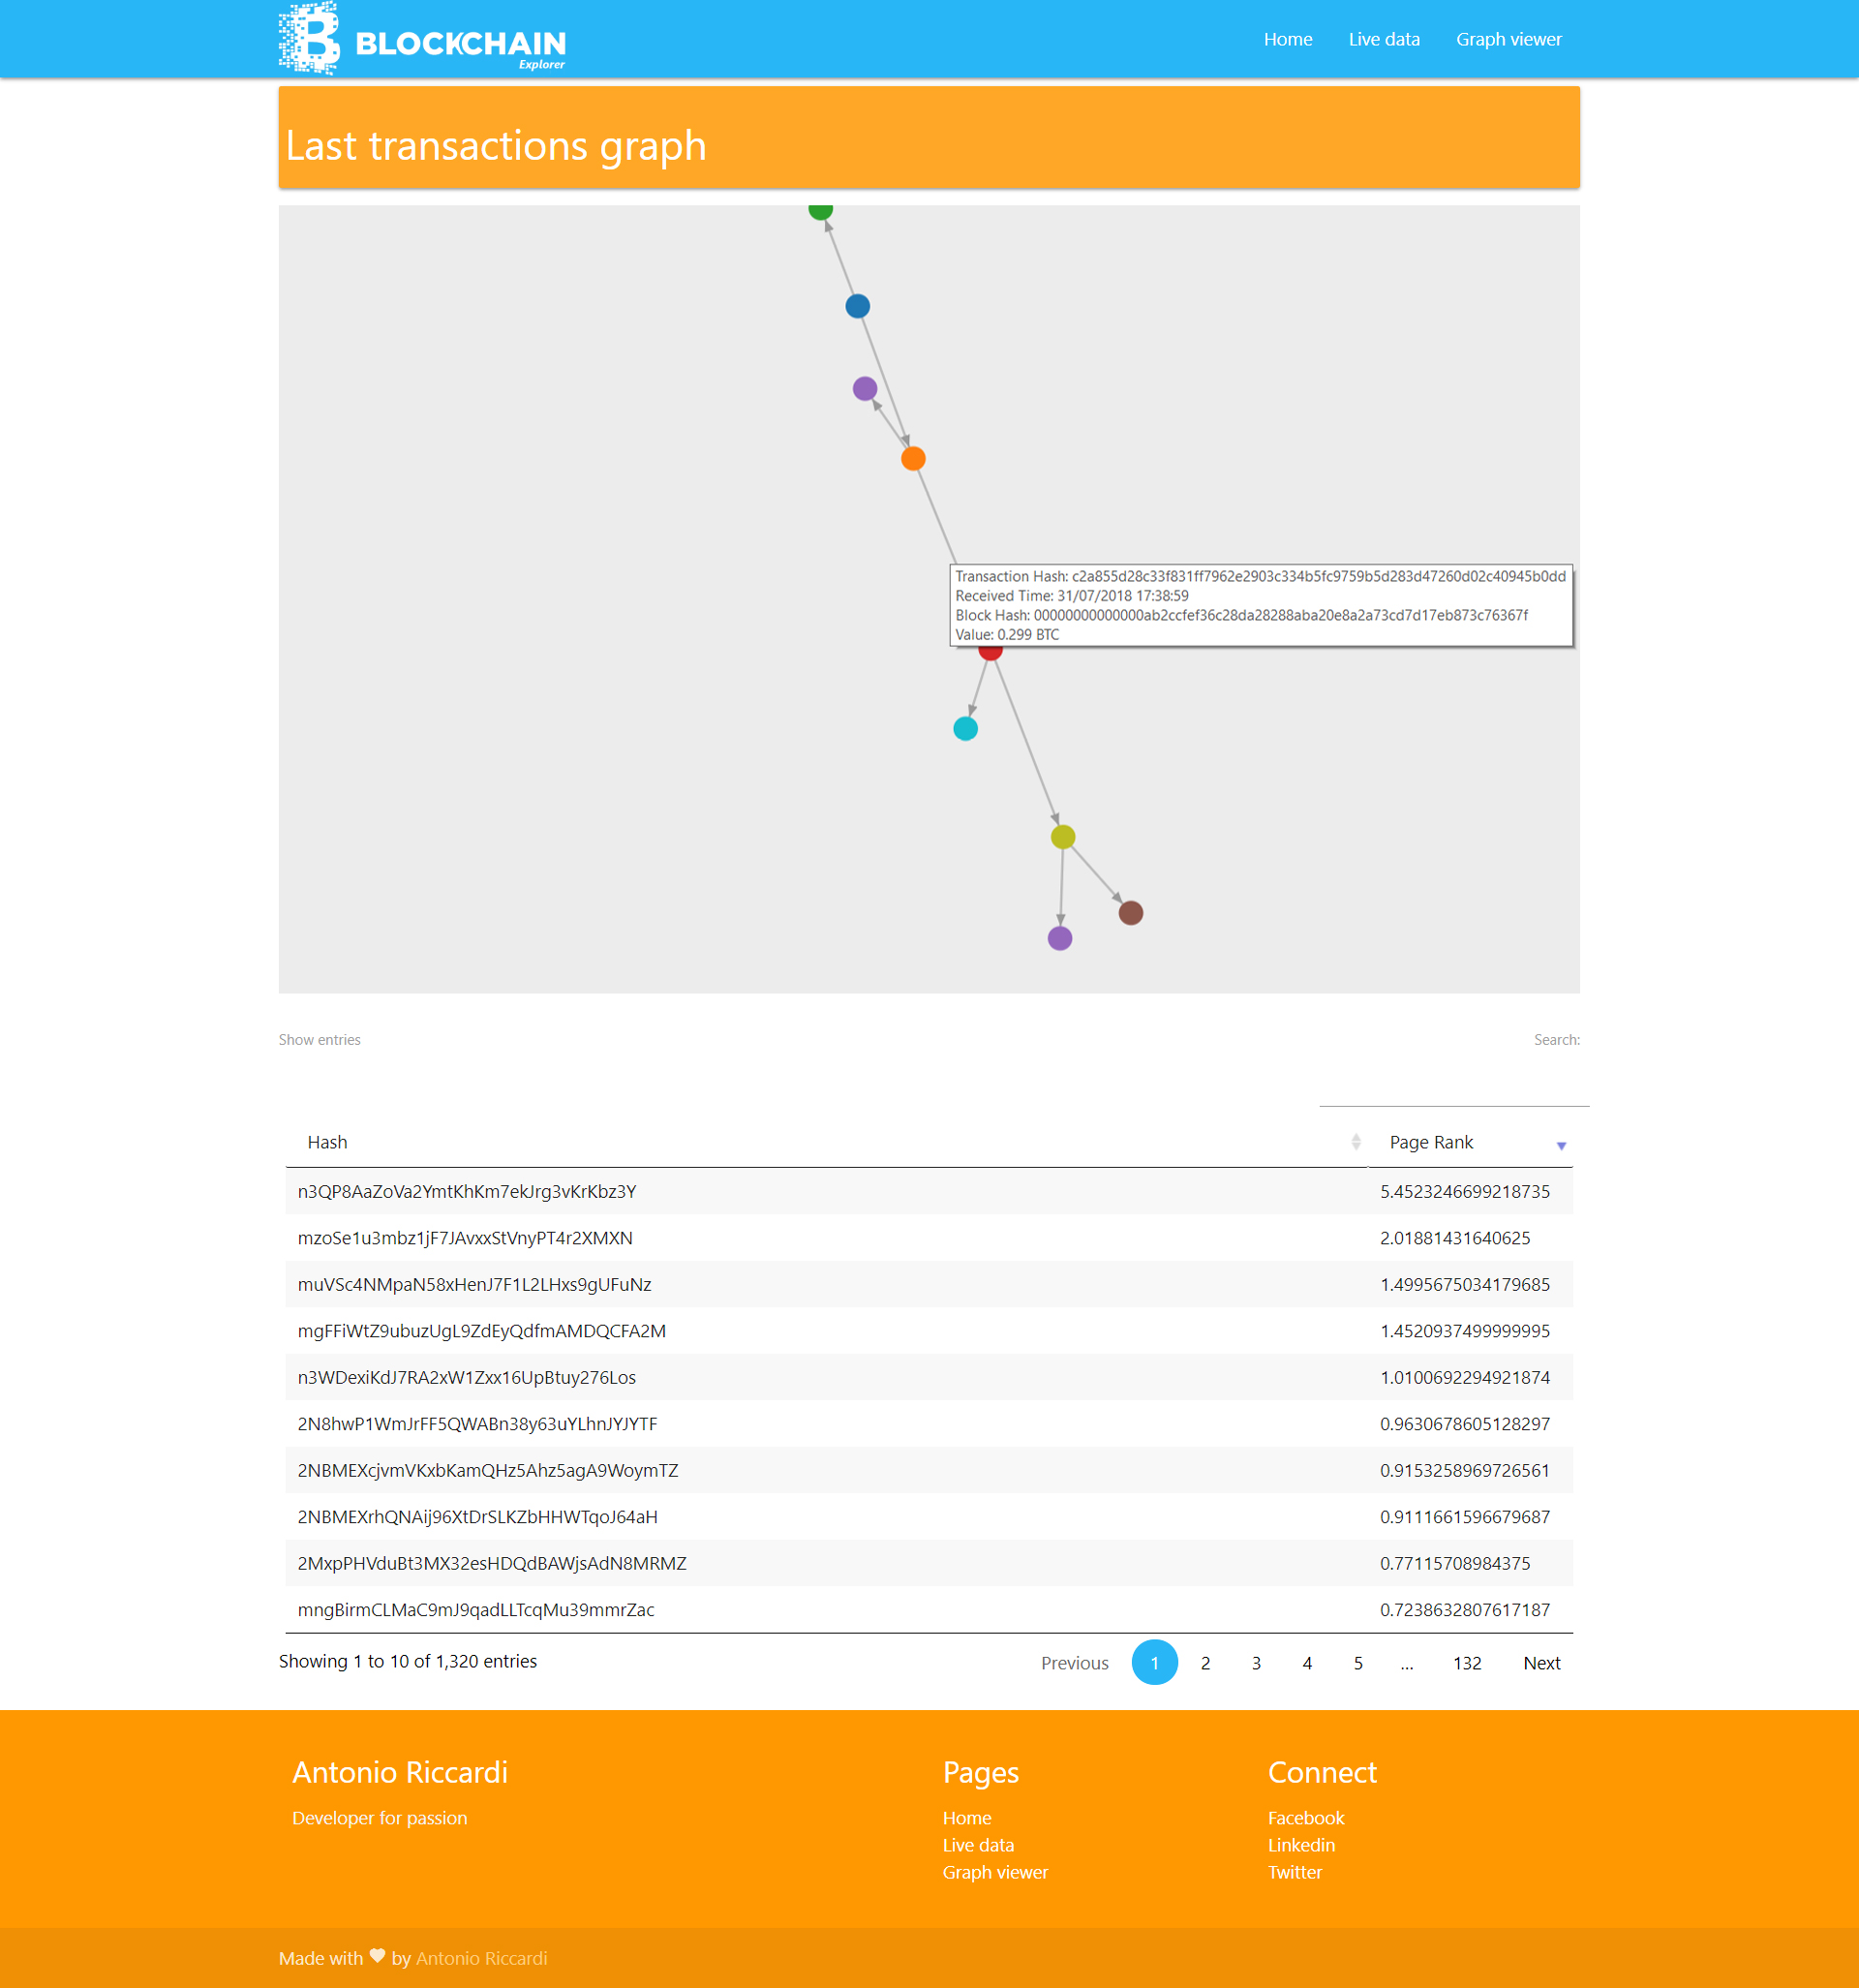
\includegraphics[width=\textwidth, height=0.80\textheight]{images/lastGraph-2.jpg}
	\caption{Dettaglio transazione all'interno del grafo.}
	\label{fig:graph2BE}
\end{figure}

\begin{figure}[H]
	\centering
	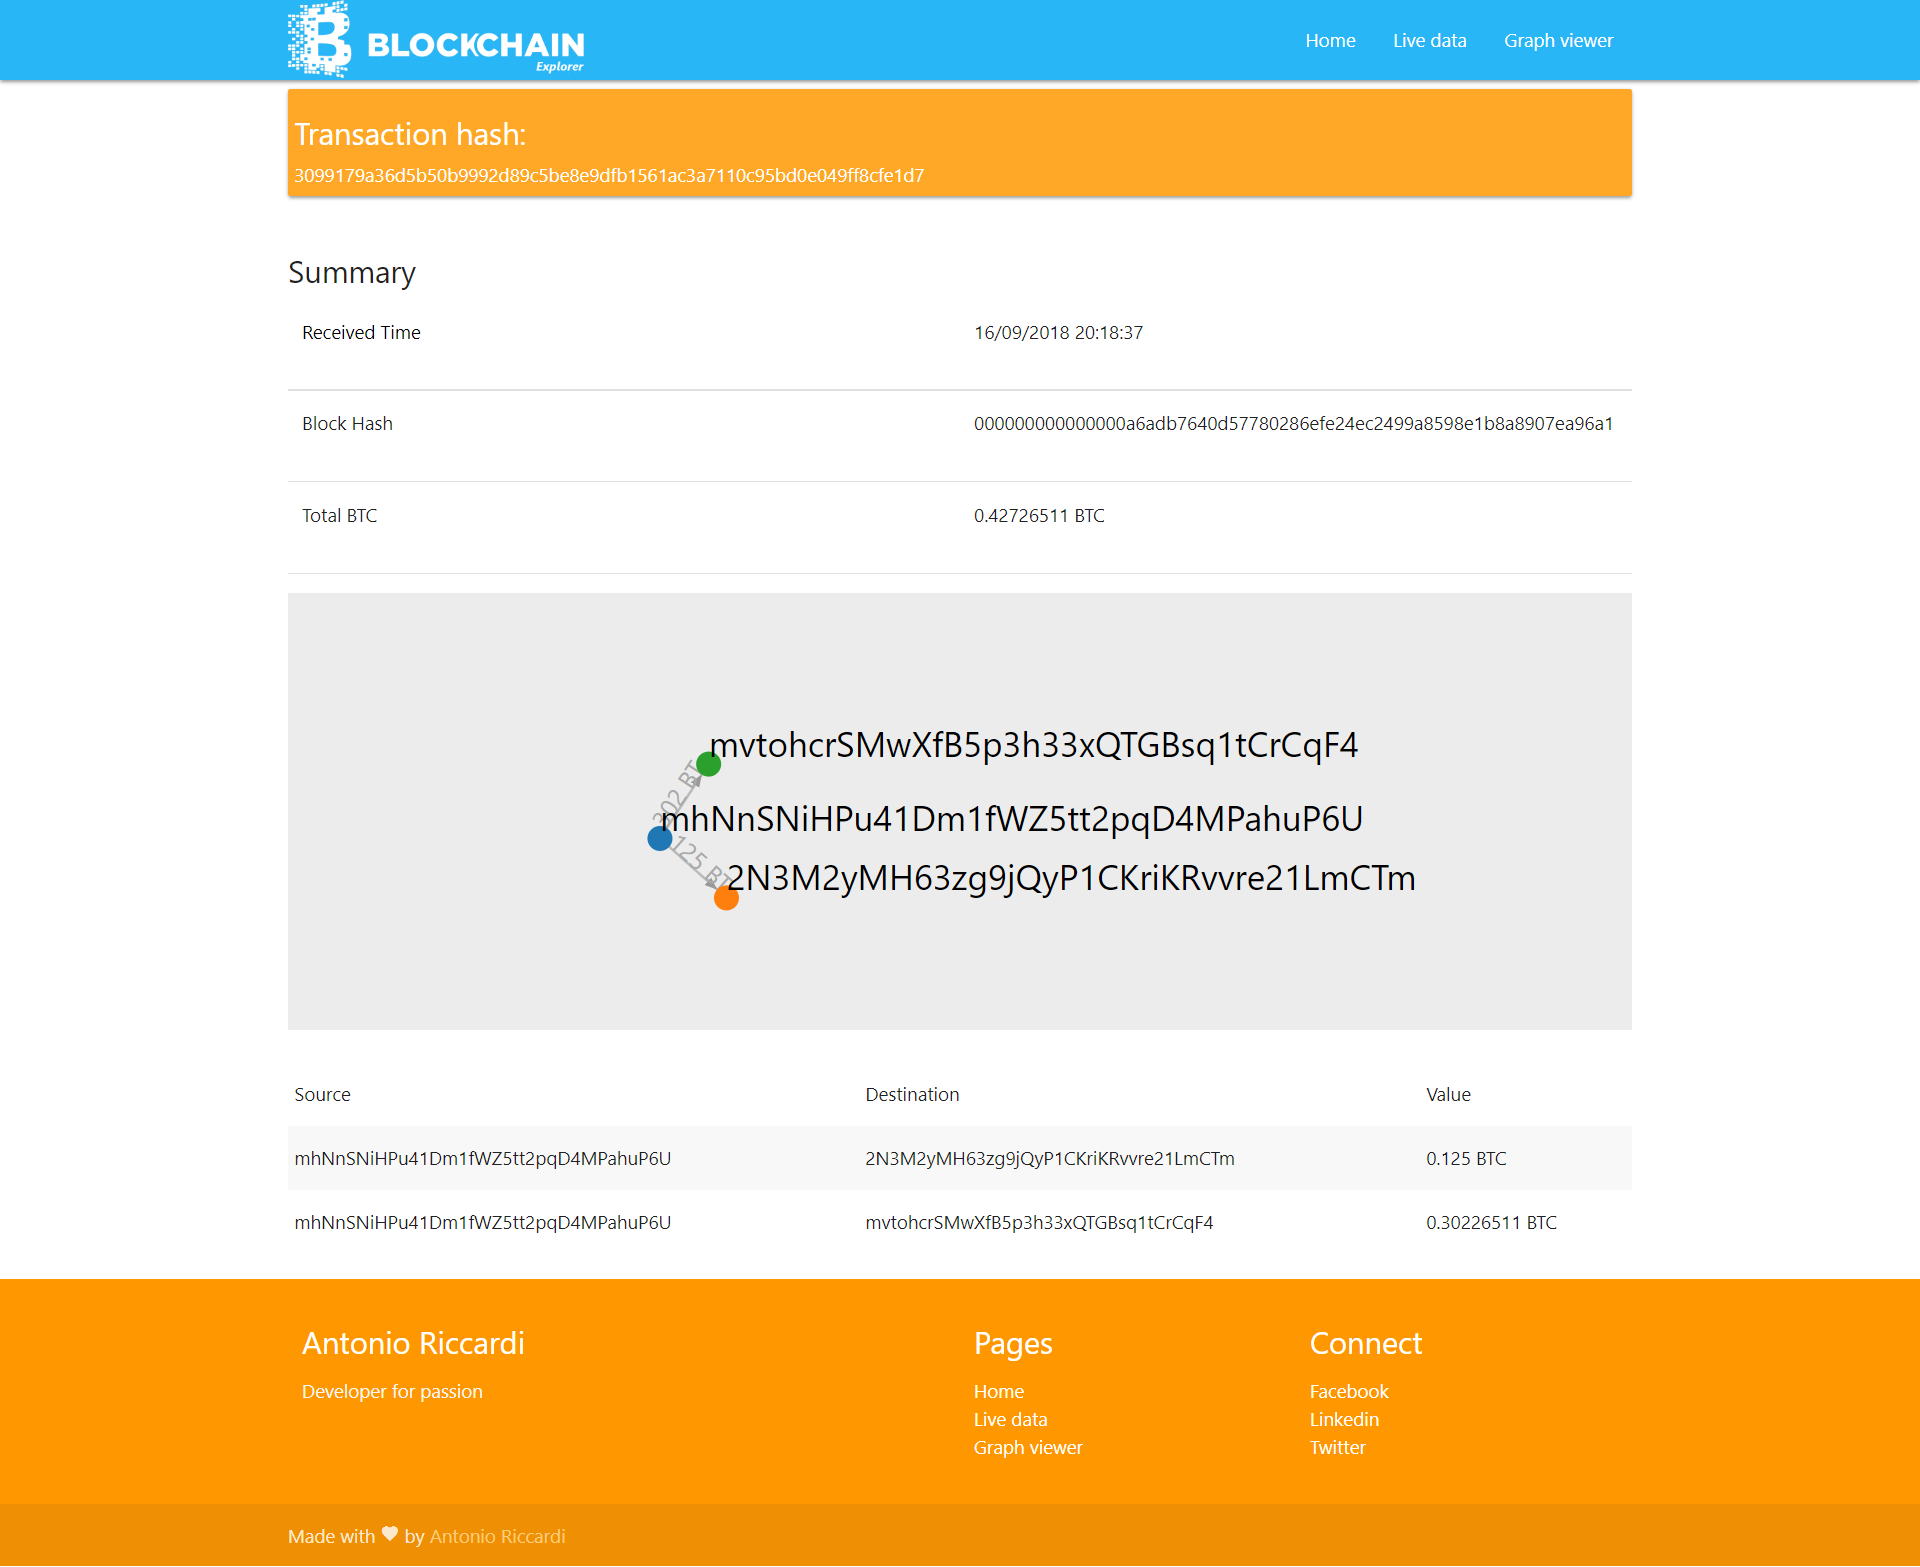
\includegraphics[width=\textwidth, height=0.80\textheight]{images/infoTransaction2.png}
	\caption{Dettaglio transazione.}
	\label{fig:detailBE}
\end{figure}

\begin{figure}[H]
	\centering
	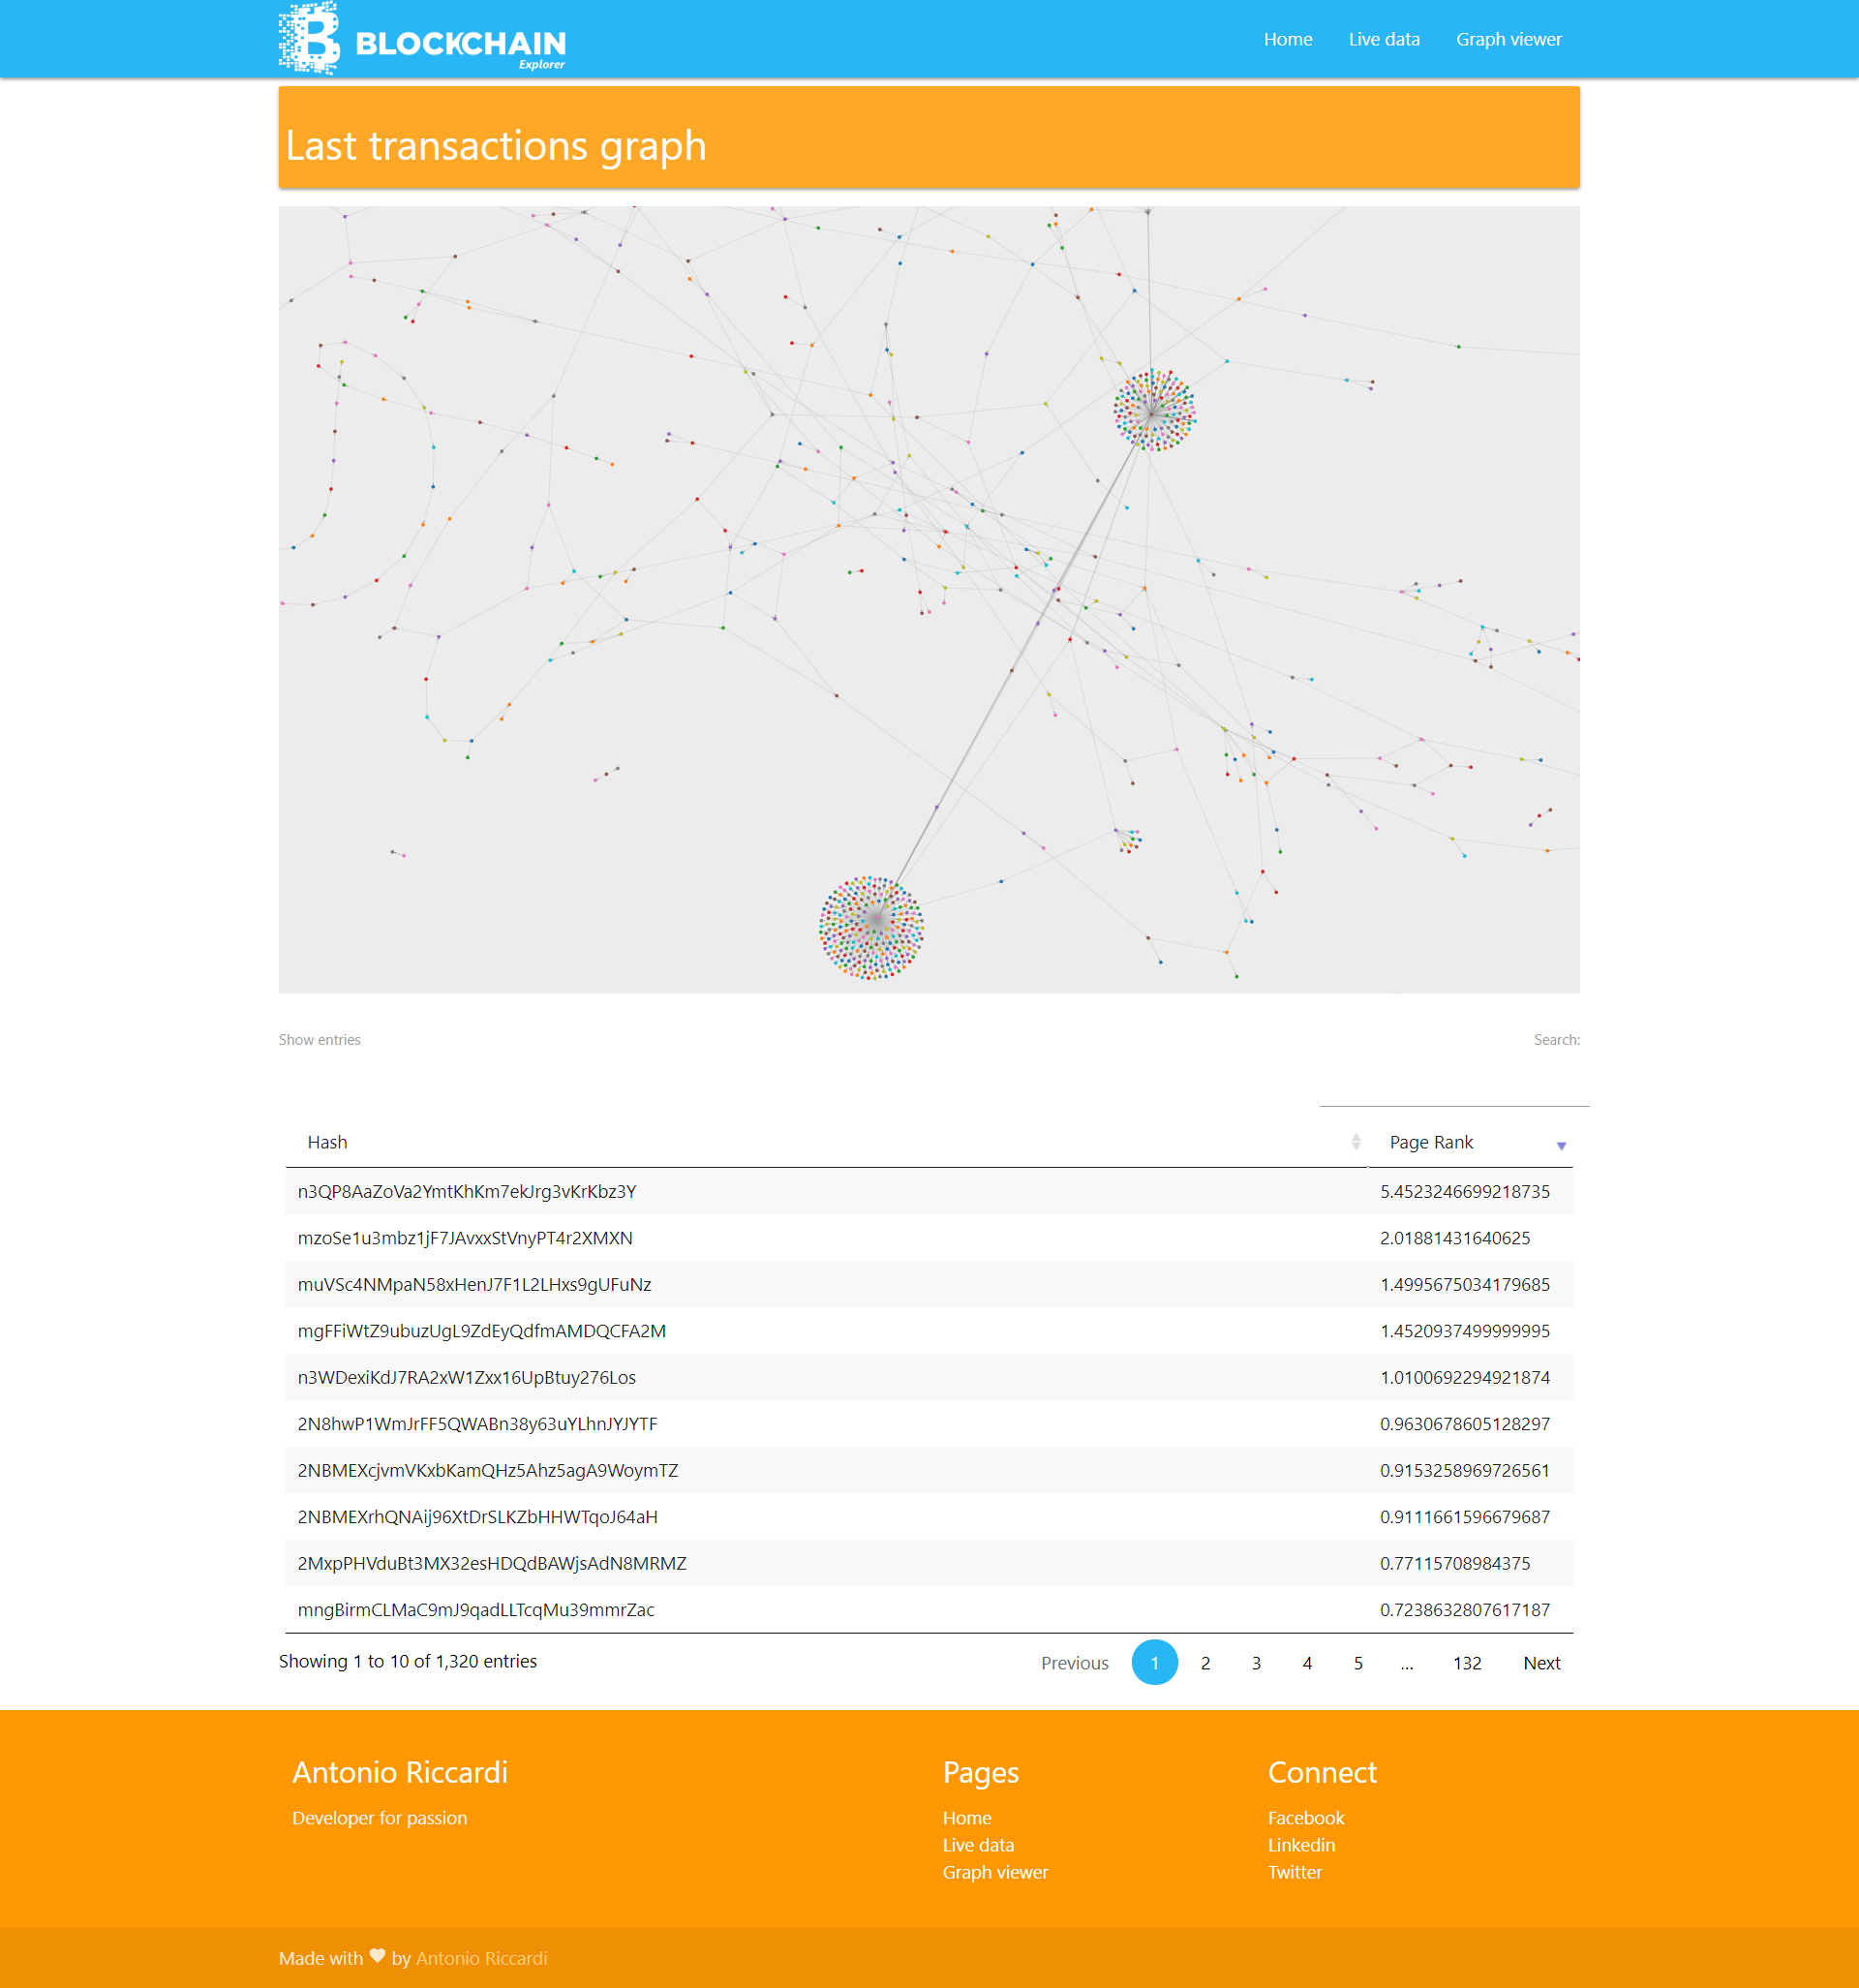
\includegraphics[width=\textwidth, height=0.80\textheight]{images/pageRankView.png}
	\caption{Visualizzazione intero grafo con calcolo del Page Rank sottostante.}
	\label{fig:graphPageBE}
\end{figure}